\documentclass[journal,12pt,twocolumn]{IEEEtran}

\usepackage{setspace}
\usepackage{gensymb}
\singlespacing
\usepackage[cmex10]{amsmath}

\usepackage{amsthm}

\usepackage{mathrsfs}
\usepackage{txfonts}
\usepackage{stfloats}
\usepackage{bm}
\usepackage{cite}
\usepackage{cases}
\usepackage{subfig}

\usepackage{longtable}
\usepackage{multirow}

\usepackage{enumitem}
\usepackage{mathtools}
\usepackage{steinmetz}
\usepackage{tikz}
\usepackage{circuitikz}
\usepackage{verbatim}
\usepackage{tfrupee}
\usepackage[breaklinks=true]{hyperref}
\usepackage{graphicx}
\usepackage{tkz-euclide}

\usetikzlibrary{calc,math}
\usepackage{listings}
  \usepackage{color}                                            %%
  \usepackage{array}                                            %%
  \usepackage{longtable}                                        %%
  \usepackage{calc}                                             %%
  \usepackage{multirow}                                         %%
  \usepackage{hhline}                                           %%
  \usepackage{ifthen}                                           %%
  \usepackage{lscape}     
  \usepackage{multicol}
  \usepackage{chngcntr}

\DeclareMathOperator*{\Res}{Res}

\renewcommand\thesection{\arabic{section}}
\renewcommand\thesubsection{\thesection.\arabic{subsection}}
\renewcommand\thesubsubsection{\thesubsection.\arabic{subsubsection}}

\renewcommand\thesectiondis{\arabic{section}}
\renewcommand\thesubsectiondis{\thesectiondis.\arabic{subsection}}
\renewcommand\thesubsubsectiondis{\thesubsectiondis.\arabic{subsubsection}}


\hyphenation{op-tical net-works semi-conduc-tor}
\def\inputGnumericTable{}                                 %%

\lstset{
	%language=C,
	frame=single, 
	breaklines=true,
	columns=fullflexible
}
\begin{document}
	
	
	\newtheorem{theorem}{Theorem}[section]
	\newtheorem{problem}{Problem}
	\newtheorem{proposition}{Proposition}[section]
	\newtheorem{lemma}{Lemma}[section]
	\newtheorem{corollary}[theorem]{Corollary}
	\newtheorem{example}{Example}[section]
	\newtheorem{definition}[problem]{Definition}
	
	\newcommand{\BEQA}{\begin{eqnarray}}
	\newcommand{\EEQA}{\end{eqnarray}}
	\newcommand{\define}{\stackrel{\triangle}{=}}
	\bibliographystyle{IEEEtran}
	\raggedbottom
	\setlength{\parindent}{0pt}
	\providecommand{\mbf}{\mathbf}
	\providecommand{\pr}[1]{\ensuremath{\Pr\left(#1\right)}}
	\providecommand{\qfunc}[1]{\ensuremath{Q\left(#1\right)}}
	\providecommand{\sbrak}[1]{\ensuremath{{}\left[#1\right]}}
	\providecommand{\lsbrak}[1]{\ensuremath{{}\left[#1\right.}}
	\providecommand{\rsbrak}[1]{\ensuremath{{}\left.#1\right]}}
	\providecommand{\brak}[1]{\ensuremath{\left(#1\right)}}
	\providecommand{\lbrak}[1]{\ensuremath{\left(#1\right.}}
	\providecommand{\rbrak}[1]{\ensuremath{\left.#1\right)}}
	\providecommand{\cbrak}[1]{\ensuremath{\left\{#1\right\}}}
	\providecommand{\lcbrak}[1]{\ensuremath{\left\{#1\right.}}
	\providecommand{\rcbrak}[1]{\ensuremath{\left.#1\right\}}}
	\theoremstyle{remark}
	\newtheorem{rem}{Remark}
	\newcommand{\sgn}{\mathop{\mathrm{sgn}}}
	\providecommand{\abs}[1]{\left\vert#1\right\vert}
	\providecommand{\res}[1]{\Res\displaylimits_{#1}} 
	\providecommand{\norm}[1]{\left\lVert#1\right\rVert}
	%\providecommand{\norm}[1]{\lVert#1\rVert}
	\providecommand{\mtx}[1]{\mathbf{#1}}
	\providecommand{\mean}[1]{E\left[ #1 \right]}
	\providecommand{\fourier}{\overset{\mathcal{F}}{ \rightleftharpoons}}
	%\providecommand{\hilbert}{\overset{\mathcal{H}}{ \rightleftharpoons}}
	\providecommand{\system}{\overset{\mathcal{H}}{ \longleftrightarrow}}
	%\newcommand{\solution}[2]{\textbf{Solution:}{#1}}
	\newcommand{\solution}{\noindent \textbf{Solution: }}
	\newcommand{\cosec}{\,\text{cosec}\,}
	\providecommand{\dec}[2]{\ensuremath{\overset{#1}{\underset{#2}{\gtrless}}}}
	\newcommand{\myvec}[1]{\ensuremath{\begin{pmatrix}#1\end{pmatrix}}}
	\newcommand{\mydet}[1]{\ensuremath{\begin{vmatrix}#1\end{vmatrix}}}
	\numberwithin{equation}{subsection}
	\makeatletter
	\@addtoreset{figure}{problem}
	\makeatother
	\let\StandardTheFigure\thefigure
	\let\vec\mathbf
	\renewcommand{\thefigure}{\theproblem}
	\def\putbox#1#2#3{\makebox[0in][l]{\makebox[#1][l]{}\raisebox{\baselineskip}[0in][0in]{\raisebox{#2}[0in][0in]{#3}}}}
	\def\rightbox#1{\makebox[0in][r]{#1}}
	\def\centbox#1{\makebox[0in]{#1}}
	\def\topbox#1{\raisebox{-\baselineskip}[0in][0in]{#1}}
	\def\midbox#1{\raisebox{-0.5\baselineskip}[0in][0in]{#1}}
	\vspace{3cm}
	\title{EE3025 ASSIGNMENT- 1}
	\author{Amgoth Hrithik Pawar - EE17BTECH11006}
	\maketitle
	\newpage
	\bigskip
	\renewcommand{\thefigure}{\theenumi}
	\renewcommand{\thetable}{\theenumi}
	Download all python codes from 
	\begin{lstlisting}
	https://github.com/AA/EE3025-IDP/tree/main/Assignment-1/codes
	\end{lstlisting}
	And Latex-tikz codes from - 
	\begin{lstlisting}
	https://github.com/AA/EE3025-IDP/tree/main/Assignment-1
	\end{lstlisting}
	\section{\textbf{Problem}}
	
	Modify the following code given in problem 2.3 with different input parameters to get the best possible output.
	\begin{lstlisting}
	import soundfile as sf
	from scipy import signal
	
	#read .wav file
	input_signal,fs = sf.read('Sound_Noise.wav')
	
	#sampling frequency of Input signal
	sampl_freq=fs
	
	#order of the filter
	order = 4
	
	#cutoff frequency 4kHz
	cutoff_freq=4000.0
	
	#digital frequency
	Wn=2*cutoff_freq/sampl_freq
	
	# b and a are numerator and denominator polynomials respectively
	b, a = signal.butter(order,Wn,'low')
	
	#filter the input signal with butterworth filter
	output_signal = signal.filtfilt(b, a, input_signal)
	#output_signal = signal.lfilter(b, a, input_signal)
	
	#write the output signal into .wav file
	sf.write('Sound_With_ReducedNoise.wav', output_signal, fs)
	
	\end{lstlisting}
	\section{\textbf{Solution}}
	The input parameters that can be modified are:
	\begin{description}[font=$\bullet$\scshape\bfseries]
		\item[]{Casacading the filter}
		\item[]{Cutoff frequency}
		
	\end{description}
	
	\subsection{\textbf{Casacading the filter}}
	 Instead of increasing the order(N) k times if we cascade the same  filter k times, we get the same response.
	 The Transfer function of k*N order Buttterworth filter is given by:
	 \begin{align}
	 H\brak{\j\omega} = \frac{1}{\sqrt{1+\brak{\frac{\omega}{\omega_{c}}}^{k*2N}}}
	 \end{align}
	 \begin{align}
	 At \frac{\omega}{\omega_{c}}>>1, |H\brak{\j\omega}|_{in dB} = -k*10N\log_{10}\brak{\frac{\omega}{\omega_{c}}}
	 \end{align}
	 Now the Transfer function of cascading k times is given by:  
	 \begin{align}
	 H\brak{\j\omega} =  \brak{\frac{1}{\sqrt{1+\brak{\frac{\omega}{\omega_{c}}}^{2N}}}}^k
	 \end{align}
	 \begin{align}
      At \frac{\omega}{\omega_{c}}>>1, |H\brak{\j\omega}|_{in dB} = -k*10N\log_{10}\brak{\frac{\omega}{\omega_{c}}}
     \end{align}

	 
	 
	\subsection{\textbf{Cutoff frequency}}
	To find a better cut-off frequency which eliminates noise, we plot all peaks in magnitude response, then take cut-off frequency which has peak above a threshold.
	The following table shows the cut-off frequency for various thresholds.
	\begin{center}
		\begin{tabular}{ |c|c| } 
			\hline
			 Thresholds & Cut-off frequency \\
			\hline
			$100$ & $4439.78$ Hz\\
			\hline
			$200$ & $4191.30$ Hz\\
			\hline
			$370$ & $3732.44$ Hz\\
			\hline
			$450$ & $2111.66$ Hz\\
			\hline
			$600$ & $2111.66$ Hz\\
			\hline


		\end{tabular}
	\end{center} 

    For threshold peak of 450 , we get 2111.66 Hz as cut-off frequency.
   \section{\textbf{Results}}
   The following plots are Frequency response of original and Filtered signals respectively.
     
\begin{figure}[!h]
	\centering
	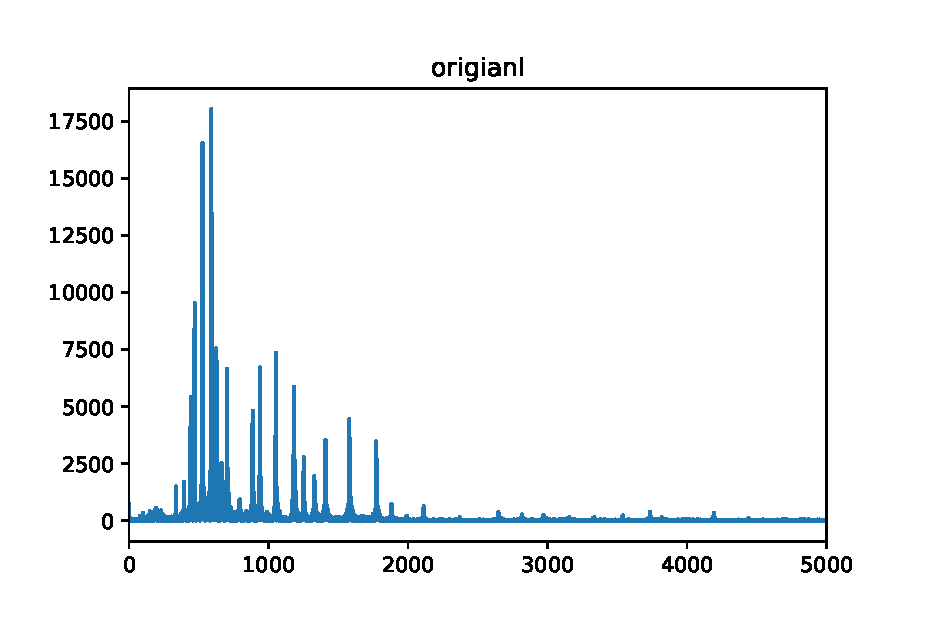
\includegraphics[width=1.2\columnwidth]{ee17btech11006_Original.eps}
	\caption{Frequency Response of Original signal}
	\label{fig:Figure1}
\end{figure} 

\begin{figure}[!h]
	\centering
	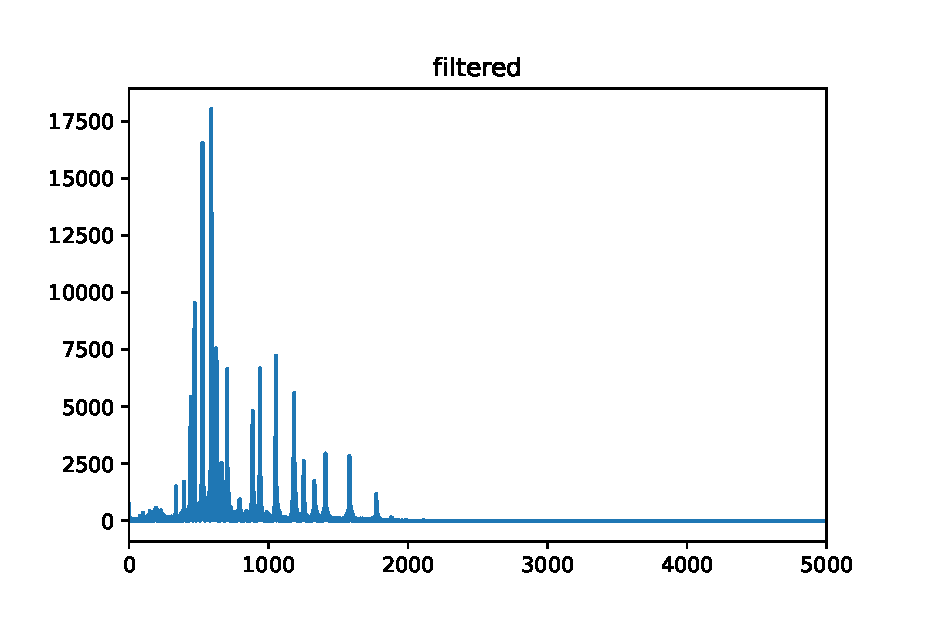
\includegraphics[width=1.2\columnwidth]{ee17btech11006_filtered.eps}
	\caption{Frequency Response of Filtered signal}
	\label{fig:Figure2}
\end{figure} 


    \section{\textbf{Summary}} 
 \begin{center}
 	\begin{tabular}{ |c|c|c| } 
 		\hline
 		Parameter & Original Signal & Filtered Signal \\
 		\hline
 		Cutoff Frequency & 4000 Hz & 2111.66 Hz \\ 
 		\hline
 		Order of filter & 4 & 4 \\
 		\hline
 		No of times  & 0 & 5 \\
 		 cascaded(filter) &  & \\
 		\hline
 		Integral of FFT & $15780177.52$ & $14417054.75$\\
 		from 0 to cutoff &  & \\
 		\hline
 		Integral of FFT & $3658619.29$ & $103996.57$\\
 		after cutoff &  & \\
 		\hline
 		Ratio of components & 0.232 & 0.007\\
 		after and before &  & \\
 		cutoff frequency &  & \\
 		\hline
 	\end{tabular}
 \end{center}

	
	
\end{document}
